% Canonical manuscript. Generated numerical inputs live in evidence/.
% Build from the repository root with make -C docs/whitepaper.
\documentclass[10pt,letterpaper,twocolumn]{article}
\usepackage[T1]{fontenc}
\usepackage{newtxtext}
\usepackage{iftex}
\ifPDFTeX
\usepackage[varqu,varl,scaled=0.95]{zi4}
\else
\setmonofont{lmmono10-regular.otf}[Scale=0.95]
\fi
\usepackage{amsmath,amssymb}
\usepackage{newtxmath}
\usepackage[letterpaper,margin=0.75in]{geometry}
\usepackage{microtype}
\usepackage{booktabs,array,tabularx}
\usepackage{xcolor}
\usepackage{tikz}
\usetikzlibrary{arrows.meta,positioning}
\usepackage{pgfplots}
\pgfplotsset{compat=1.18}
\usepackage{fancyhdr}
\usepackage{titlesec}
\usepackage{needspace}
\usepackage{balance}
\usepackage{url}
\usepackage[numbers]{natbib}
\definecolor{ink}{HTML}{214E70}
\definecolor{accent}{HTML}{B85C38}
\definecolor{pale}{HTML}{F3F5F7}
\usepackage[colorlinks=true,linkcolor=ink,citecolor=ink,urlcolor=ink]{hyperref}
\hypersetup{pdftitle={Limit Order Book: A Price-Time Priority Matching Engine for C++, C, and Python},pdfauthor={Christian Kauten},pdfsubject={Project technical report; revision October 19, 2026},pdfkeywords={limit order book, price-time priority, matching, C++, C, Python, reproducible evaluation}}
\setlength{\columnsep}{0.25in}
\setlength{\headheight}{14pt}
\setlength{\emergencystretch}{1.5em}
\titleformat{\section}{\large\bfseries\raggedright}{\thesection}{0.6em}{}
\titleformat{\subsection}{\normalsize\bfseries\raggedright}{\thesubsection}{0.6em}{}
\titlespacing*{\section}{0pt}{2.2ex plus 0.5ex minus 0.2ex}{1ex}
\titlespacing*{\subsection}{0pt}{1.7ex plus 0.4ex minus 0.2ex}{0.7ex}
\raggedbottom
\pagestyle{fancy}
\fancyhf{}
\fancyhead[L]{\small\textsc{Limit Order Book}}
\fancyhead[R]{\small Technical report / October 2026}
\fancyfoot[C]{\thepage}
\newcommand{\code}[1]{\texttt{#1}}
\makeatletter
\newcommand{\studyrows}{\@@input evidence/table-rows.tex }
\makeatother
% Generated from timings.csv by evaluate.py --summarize.
\newcommand{\StudyAscLast}{4359.6}
\newcommand{\StudyDescLast}{4491.1}
\newcommand{\StudyShuffleLast}{105.7}
\newcommand{\StudyPairCpp}{44.4}
\newcommand{\StudyPairC}{45.3}
\newcommand{\StudyFifoLast}{4333.9}
\newcommand{\StudyLevelsLast}{9455.4}
\newcommand{\StudyClock}{15.6}
\newcommand{\StudyInsertionRatio}{41.2}

\title{\textbf{Limit Order Book: A Price-Time Priority\\Matching Engine for C++, C, and Python}}
\author{Christian Kauten}
\date{Technical report revision: October 19, 2026}

\begin{document}
\twocolumn[\maketitle
\begin{abstract}
\noindent
\emph{Limit-order-book} turns an established price-time matching design into
a compact C++ library with C and Python interfaces. The construction gives
each access pattern its own representation: a tree orders occupied prices,
intrusive FIFO queues preserve arrival priority, hash indices locate orders
and levels, and cached pointers and aggregates answer common queries. This
organization follows the 2011 \emph{How to HFT} account and was present in the
project's first commit in December 2019. Historical engine sources included
with that commit illustrate alternatives: a bounded price array and order
arena in voyager's QuantCup submission, and indexed records with reuse in
Joshua Levine's Island2. We explain why the library's combination is useful
for sparse integer prices, direct cancellation, and reuse across applications,
and how its first-party tree and list work with the vendored hash map. These
benefits have specific limits: the tree is unbalanced, allocation remains on
mutation paths, and explicit lifetime discipline is required. An archived
study of an earlier source snapshot supports the analysis with 200,000
model comparisons and repeated C++/C timings on one Apple M1 Pro. It finds
stable existing-level update costs across the tested depths and strong
insertion-order sensitivity. The study characterizes this design; it is not
a ranking against the historical engines or a measurement of later dependency
updates.
\end{abstract}
\par\vspace{0.7em}
\noindent\textbf{Keywords:} limit order book; price-time priority; matching;
intrusive data structures; language interfaces; reproducible measurement.
\par\vspace{1.4em}
]

\section{Introduction}
A useful limit order book must answer several different questions about the
same orders. Matching needs the best eligible price and the oldest order at
that price. Cancellation needs an order by identifier. A strategy may need
inside prices or accumulated volume without walking the book. Putting every
operation through one sorted container would make some of these questions
more expensive than necessary. The design used here combines specialized
views while keeping one order object and one node for each occupied price.

The \emph{limit-order-book} project implements that organization for one
instrument~\cite{kauten-limit-order-book-2019}. Incoming limit orders cross
eligible opposing liquidity and rest any remainder; market orders consume
liquidity without resting. The current implementation is a header-only C++14
library with separate C and Python bindings. Applications supply event
sequencing and the surrounding simulation or trading infrastructure.

The engineering value lies in how the parts fit together. A hash lookup and
intrusive links make an existing-level update independent of the price tree.
A price tree represents only occupied prices, without reserving an array for
the numeric tick range. Cached best pointers and incremental aggregates make
frequent state queries direct reads. A shared native core keeps the matching
policy in one place across language interfaces. These are concrete reasons
for choosing this organization, with costs in pointers, allocation, and the
need to maintain agreement between indices.

This report first places the design in its historical context, then follows
its construction from nodes to matching operations and language interfaces.
The detailed behavior, complexity analysis, and archived evaluation establish
where those benefits hold. The report explains an implementation of known
ideas; it does not introduce a new matching policy or claim a universally
fastest representation.

\section{Design Context: What Was Already Known}
\subsection{The 2011 design and the 2019 implementation}
The \emph{How to HFT} article ``How to Build a Fast Limit Order Book,'' dated
February 15, 2011, describes one tree per side, a doubly linked queue per
price, order-ID and price indices, and cached inside prices~\cite{howtohft}.
Its central insight is to organize the book around the operations that need
to be cheap. Finding an order, ordering prices, and maintaining time priority
are different jobs. The repository preserves an attributed transcription;
the original site was unavailable during this review.

The project's initial commit, \code{c0dfd34} (December 16, 2019), already
contains these notes, both historical engine files discussed below, and the
core tree/queue/hash organization. Its headers use intrusive \code{Order} and
\code{Limit} nodes, \code{std::unordered\_map} for order values, and
\code{tsl::robin\_map} for price-to-limit pointers. This gives a verifiable
historical frame: those ideas and examples were present when this codebase
began. It does not imply that the initial API, quantities, or ownership
behavior were identical to today's implementation. Exact Git paths and
source provenance are recorded in the accompanying source map.

The article also calls for keeping the price tree balanced. The project uses
an ordinary binary search tree, so it implements the organization without
that guarantee. The distinction is central to evaluating the design fairly:
existing-level updates can bypass the tree, but new-level insertion still
depends on its height. Section~\ref{sec:complexity} derives the actual costs.

\subsection{Alternative engineering choices in the reference engines}
The QuantCup~1 source credits \emph{voyager}~\cite{quantcup}. A fixed
\code{pricePoints} array indexes queues by numeric price; a contiguous
\code{arenaBookEntries} array supplies order storage. Tail insertion
preserves arrival order. Cancellation marks an entry's size zero, leaving
matching to pass over it later. This construction avoids per-order heap
allocation and makes locating a price an array access. It also commits to a
bounded price range and arena, and scans price slots when seeking liquidity.
Its advantages are plausible for the constrained simulated feed described in
the source; the comments are not evidence of performance on arbitrary books.

Our representation makes a different tradeoff. It allocates nodes only for
occupied prices, accepts caller-supplied integer IDs, and unlinks cancelled
orders immediately. Memory need not scale with the numeric gap between two
prices, and later matching need not walk cancelled queue entries. In return,
it pays for hash tables, pointers, and dynamic allocation. A dense, bounded
price grid or an arena can be a better choice for a suitably constrained
workload. The local QuantCup file is undated; its presence in the 2019 commit
establishes availability to this project, not a contest ranking or a precise
publication date.

Joshua Levine's \emph{Island2} source identifies version 2.40 and carries a
1996 copyright notice~\cite{island}. The release page describes a December 15,
2003 FoxPro snapshot; the notice alone does not date the local copy. Its
matching procedure selects opposing records through database indices, handles
partial fills and quantity conditions, emits messages, and places depleted
records on a reuse list. Levine describes indexing and messaging support
outside that procedure. The useful lesson is architectural: a short matching
loop can rely on substantial storage and integration machinery. This library
puts its indices in C++ and leaves external sequencing, messaging, and
persistence to its caller. It does not provide Island's surrounding system.

Table~\ref{tab:design-context} summarizes the tradeoffs visible in the sources.
Neither historical engine is compiled or timed here, and the comparison does
not establish direct code ancestry. Their original attribution and licensing
scope remain separate from the project's first-party implementation.

\begin{table*}[t]
\centering\small
\begin{tabularx}{\textwidth}{@{}>{\raggedright\arraybackslash}p{0.16\textwidth}
 *{3}{>{\raggedright\arraybackslash}X}@{}}
\toprule
Design or source & Representation & Useful consequence & Cost or condition\\
\midrule
How to HFT (2011) & Price trees, per-price queues, hash indices & Different
access paths for matching, cancellation, and queries & Logarithmic tree work
requires a balancing strategy\\
\addlinespace
voyager / QuantCup & Price array, fixed order arena, singly linked queues &
Direct price indexing; no per-order heap allocation & Bounded range and
capacity; scans and deferred cancellation work\\
\addlinespace
Levine / Island2 & Indexed records, depleted-record reuse, messaging calls &
Small matching procedure supported by reusable records and indices & Depends
on database and supporting runtime absent from the local excerpt\\
\addlinespace
This library & Occupied-price tree, intrusive queues, two hash indices &
Sparse price storage; direct unlinking; cached best and aggregates & Dynamic
allocation; unbalanced tree; explicit lifetime constraints\\
\bottomrule
\end{tabularx}
\caption{Source-based design comparison, not a throughput ranking. The
historical examples were already included in the project's first commit.
The last row describes the implementation inspected for this revision.}
\label{tab:design-context}
\end{table*}

\subsection{Current components and the measured snapshot}
Christian Kauten's tree and list helpers now live in \path{include/} under
\code{LOB::BST} and \code{LOB::DLL}~\cite{bst,dll}. Their October 2026
integration makes them first-party components maintained with the matching
engine and its tests. It preserves the intrusive representation; moving the
sources and namespacing them does not balance the tree or imply a speedup.

The remaining vendored component is Tessil's \emph{robin-map}, which uses
open addressing, Robin Hood probing, and backward-shift deletion~\cite{robin}.
The current vendoring pins v1.3.0, commit \code{188c45569cc2}, with upstream
headers, license, and file checksums. This is a later maintenance choice,
not the version used by the original 2019 implementation. Cython bindings
and the current CMake distribution are likewise later developments.

The archived study uses base revision \code{3a4d254e9bda}, with exact
implementation and study inputs identified by SHA-256 manifests. It predates
the helper integration and the v1.3.0 update. Its earlier tree/list paths and
hash-map bytes remain in the archive. The architecture discussion follows
the current source where these choices persist; every numerical result in
this report belongs to the archived snapshot. No result is relabeled as a
measurement of the updated dependency.

\section{Behavioral Model}
\subsection{Prices, quantities, and priority}
An order has an identifier, side, remaining quantity, and limit price.
Identifiers and prices use unsigned 64-bit integers; individual quantities
and order counts use unsigned 32-bit integers; aggregated volume uses an
unsigned 64-bit integer. A price is an integer tick value with a scale chosen
by the caller. The implementation does not perform currency conversion or
floating-point price comparison.

Let $p_b$ denote a buy limit and $p_a$ a sell limit. They can match when
$p_b\geq p_a$. Among resting sells, the lowest eligible price executes first;
among resting buys, the highest executes first. At a common price, the oldest
remaining order executes first. ``Time'' is represented by queue position,
not by a timestamp field or a wall-clock reading. Calls must therefore arrive
in the sequence the application intends to model.

For an incoming remaining quantity $q$ and resting quantity $r$, a matching
step removes $\min(q,r)$ from both. A zero remaining resting quantity causes
the order to leave the queue and identifier map immediately. A positive
remainder stays in the same queue position. A crossing limit continues until
it is filled, no eligible price remains, or the opposing side is empty; its
unfilled remainder then joins its own side. An unfilled market remainder is
discarded when the call returns.

The implementation uses price zero internally to mean an unrestricted market
price and returns zero for an empty side's best-price query. The evaluated
domain therefore uses strictly positive limit prices and quantities. The
public methods do not comprehensively validate this domain. Treating zero
as an ordinary priced limit would conflate different meanings and is outside
the report's correctness claim.

\subsection{A matching example}
Consider resting sells $A=(101,5)$, $B=(101,7)$, and $C=(102,4)$, in that
arrival order, where each pair is (price, quantity). A buy limit for nine at
101 fills all five units of $A$ and four units of $B$. The remaining state is
$B=(101,3)$ and $C=(102,4)$; the buy does not rest. The best ask stays 101,
total sell volume becomes seven, and the identifier for $A$ is absent.

A subsequent market buy for five fills the remaining three units of $B$,
removes the now-empty 101 level, and fills two units of $C$. The best ask
becomes 102 and $C$ retains two units. This trace illustrates why matching
correctness concerns the residual order identities as well as aggregate
volume: reversing $A$ and $B$ could preserve the totals while violating FIFO.

\subsection{Identifier and update semantics}
A new limit with an already-live identifier is ignored before crossing or
queue insertion, including when the submitted side or price differs. An
identifier can be reused after its order fills, is cancelled, or is cleared.
A market order's identifier is carried in a temporary object and is not
registered as a resting order. It does not provide an execution-record key.

Cancellation removes an entire resting order. The C++ \code{reduce} method
subtracts quantity while preserving arrival priority, and cancels the order
when its remaining quantity reaches zero. Increasing an order or replacing
its price is not a supported primitive. A caller that cancels and resubmits
creates a new arrival position.

Unknown identifiers illustrate a boundary difference: C++ lookup and
cancellation use \code{orders.at} and can throw; the C and Python cancellation
wrappers ignore unknown identifiers. The C lookup returns a null pointer for
an unknown identifier. The interfaces share a matching core but do not expose
every C++ method or identical failure behavior. In particular, reduction and
several last-price queries are C++ operations in the inspected interfaces.

\section{Building the Book from Intrusive Components}
\subsection{Indices and intrusive links}
Figure~\ref{fig:architecture} summarizes the organization. An \code{Order}
derives from a doubly linked list node. Its predecessor and successor are
part of the order object, and it carries a pointer to its containing
\code{Limit}. A limit derives from a binary search tree node and stores its
queue head and tail, order count, and total quantity. The first-party helpers
manipulate these embedded links; they do not allocate a second list or tree
wrapper for each object. The node owner remains responsible for storage.

\begin{figure}[t]
\centering
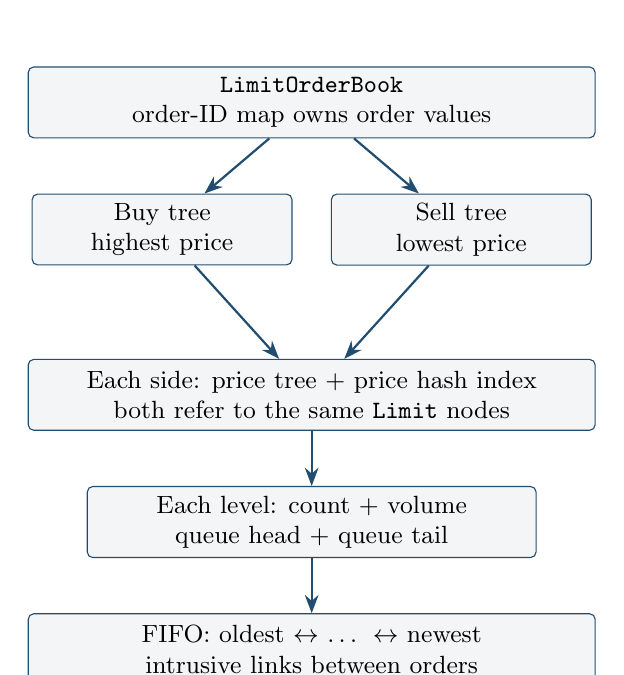
\begin{tikzpicture}[font=\small,>=Stealth,
 box/.style={draw=ink,rounded corners=2pt,fill=pale,align=center,minimum height=9mm},
 link/.style={->,draw=ink,thick}]
\node[box,minimum width=72mm] (book) {\code{LimitOrderBook}\\order-ID map owns order values};
\node[box,below=7mm of book,xshift=-19mm,minimum width=33mm] (buy) {Buy tree\\highest price};
\node[box,below=7mm of book,xshift=19mm,minimum width=33mm] (sell) {Sell tree\\lowest price};
\node[box,below=28mm of book,minimum width=72mm] (levels) {Each side: price tree + price hash index\\both refer to the same \code{Limit} nodes};
\node[box,below=7mm of levels,minimum width=57mm] (limit) {Each level: count + volume\\queue head + queue tail};
\node[box,below=7mm of limit,minimum width=72mm] (queue) {FIFO: oldest $\leftrightarrow$ \dots{} $\leftrightarrow$ newest\\intrusive links between orders};
\draw[link] (book) -- (buy);
\draw[link] (book) -- (sell);
\draw[link] (sell) -- (levels);
\draw[link] (levels) -- (limit);
\draw[link] (limit) -- (queue);
\draw[link] (buy) -- (levels);
\end{tikzpicture}
\caption{Both sides use the representation expanded below the side boxes.
Order storage belongs to the identifier map; price levels are separately
allocated. Cached best pointers and aggregates avoid searches for common
queries. The arrows denote composition, not order flow between sides.}
\label{fig:architecture}
\end{figure}

Each \code{LimitTree<Side>} contains a tree root, price-to-limit hash index,
cached best pointer, and side-wide count and volume. The template parameter
selects side-specific comparisons. The enclosing \code{LimitOrderBook}
contains both sides and the order-ID index. Crossing orders use the opposing
tree's matching routine; a templated callback erases completely filled order
IDs from the enclosing map.

The order map stores order values in its nodes. Stable addresses across
rehashing are important because queues hold pointers to those values. The
price map stores pointers to separately allocated limits, so movement of
entries within that hash table does not move the tree nodes. This distinction
explains why replacing one container with another requires a lifetime audit
as well as a timing comparison.

\subsection{Why the access paths are separate}
A noncrossing order at an existing price reaches its level through the price
hash index and appends through the cached queue tail. No price-tree search or
queue traversal is needed. On cancellation, the ID map supplies the order,
its back-pointer supplies the level, and its previous/next links supply its
neighbors. Removing a middle order therefore does not search the queue.
The extra predecessor pointer earns its space on this cancellation path.

The queue's head encodes the next order to execute. A partial fill changes
quantity while leaving that position intact. This represents time priority
structurally, without sorting timestamps on every match. It also makes the
caller responsible for the sequence in which operations arrive. Level and
side counts and volumes are updated with each mutation, exchanging a few
writes for constant-time reads of those stored aggregates. Arbitrary price
range sums are not supplied by these aggregates.

The two hash maps have different storage duties. The order map owns objects
whose addresses must survive rehashing; the price map holds pointers to
separately allocated tree nodes. Robin Hood insertion and backward-shift
erasure may relocate hash-table entries, but moving a stored \code{Limit*}
does not move its target. The vendored map is therefore suitable for the
price index without assuming stable addresses inside its buckets. Replacing
the order map with the same flat container while retaining order values
inline would invalidate the queue's lifetime assumptions. This is a
representation constraint, not evidence that one hash table is always faster.

Finally, \code{LimitTree<Side>} expresses the two sides with shared queue and
matching logic and side-specific comparisons. The outer book handles IDs
and crossing; the side handles price eligibility and fills; the node helpers
handle links. This division keeps a small implementation inspectable while
allowing C and Python to use the same native matching behavior.

\subsection{Invariants and update order}
For each live level $\ell$, with queue $Q_\ell$, the intended aggregates are
\begin{equation}
 c_\ell=|Q_\ell|,\qquad
 v_\ell=\sum_{o\in Q_\ell}q_o.
\end{equation}
Side-wide count and volume are the corresponding sums across its levels.
A nonempty side's cached best pointer identifies its extreme price; an empty
side has a null best pointer. Every live order appears exactly once in the
identifier map and exactly once in a price queue. Every live level appears
in the tree and price index and has a nonempty queue.

An insertion at an existing price appends to the tail and updates aggregates.
An insertion at a new price allocates a limit, inserts it in the tree and
price index, and updates the best pointer if necessary. Cancelling a nonfinal
order unlinks it from the queue. Cancelling the last order removes the price
node and its index entry, updates the best pointer when needed, and deletes
the limit. The caller erases the order from the identifier map afterward.

A partial fill adjusts the resting quantity, level volume, and side volume
without changing queue position or count. A full fill uses the cancellation
path before invoking the callback that erases the order's map entry. The
ordering of these actions avoids destroying the order while its links are
still needed for removal.

\subsection{Lifetime boundaries}
The inspected C++ types allocate levels with \code{new} and release them in
\code{clear} or when their final order leaves. They do not provide an owning
destructor that clears outstanding levels. Ordinary destruction of a nonempty
book therefore does not reclaim those level allocations. The C deletion
function likewise deletes its wrapper without first clearing the book.
This is an implementation limitation, not a property concealed by the
benchmark: the study explicitly clears every residual book outside timing.
The Cython wrapper clears before deleting its native object.

The C++ types also retain implicit copying despite containing raw links.
Copying a populated book does not reconstruct an independent graph of its
orders and levels. The report and study use one owner per book and do not
exercise copying. Production ownership improvements would require a separate
change and validation; none is made to obtain these measurements.

\section{Operation Costs}\label{sec:complexity}
Let $N$ be the number of live orders, $M$ the number of price levels on a side,
and $h$ that side's tree height, counting nodes on the longest root-to-leaf
path. Table~\ref{tab:complexity} separates tree work
from hash-table assumptions. Hash lookup costs below are expected, and table
growth is amortized; adversarial collisions, allocation, and rehashing prevent
these expressions from being hard latency guarantees. Let $B$ denote retained
hash-bucket capacity, which can exceed the current live population.

\begin{table}[t]
\centering\small
\begin{tabularx}{\columnwidth}{@{}Xl@{}}
\toprule
Operation or condition & Structural cost\\
\midrule
Read cached best, count, or volume & $O(1)$\\
Find order or level by hash index & Expected $O(1)$\\
Add at an existing, noncrossing level & Expected amortized $O(1)$\\
Add a new, noncrossing level & $O(h)$ + hash work\\
Cancel while the level remains live & Expected $O(1)$\\
Cancel the final order at a level & Up to $O(h)$ + hash work\\
Match $k$ orders, erase $d$ levels & $O(k+dh)$ + hash work\\
Clear the book, including bucket scans & $O(N+M+B)$\\
\bottomrule
\end{tabularx}
\caption{Costs of the inspected implementation. The sweep expression is a
conservative bound using the maximum encountered height. A crossing limit
also pays for resting any remainder. Allocation costs are not bounded here.}
\label{tab:complexity}
\end{table}

\subsection{Tree height is not controlled}
The underlying insertion procedure follows child pointers until it reaches
an empty link. It does not rebalance. Sorted distinct prices create a chain
with $h=M$, so the next insertion can take linear time in the number of
levels. Building $M$ levels this way visits
\begin{equation}
 \sum_{i=0}^{M-1}i=\frac{M(M-1)}{2}
\end{equation}
existing nodes during insertion. Dividing by $M$ yields a linearly growing
amount of tree work per order. A logarithmic claim is conditional on the
tree remaining shallow, not an invariant maintained by this implementation.

Caching the best pointer makes reading the inside price constant-time; it
does not make every update to that pointer constant-time. When an extreme
level disappears, \code{find\_best} can traverse to a minimum or maximum in
the remaining subtree. Removing a nonextreme node with two children can also
search for a successor. The final-order cancellation case must therefore
remain separate from unlinking an order whose level survives.

\subsection{A market request can contain many executions}
The matching loop visits resting orders until the incoming quantity is
exhausted or no eligible liquidity remains. Filling one resting order is not
the same unit of work as processing one market request. If a request fills
$k$ resting orders and deletes $d$ price levels, both quantities matter.
In particular, a sweep of a long queue at one price and a sweep with one
order at each of many prices can trade the same total quantity while causing
different structural work. Section~\ref{sec:results} measures this distinction.

\section{Language and Distribution Boundaries}
The C++ library is header-only and requires C++14. Its CMake target is
\path{limit_order_book::limit_order_book}. Installed headers include the
tree and list components and the vendored \emph{robin-map} library.
A default subproject does not build the
study, tests, or language bindings. Packaging is part of the reproducibility
surface, but successful installation alone is not evidence of matching
correctness or speed.

The C99-compatible header exposes a forward-declared book handle and fixed
width scalar aliases. Definitions in a separate translation unit forward to
the C++ book, with compile-time checks on the scalar type correspondence.
The optional \code{limit\_order\_book::c} target builds this bridge. The report's
C timing experiment loads a separately compiled shared library, so the bridge
is not inlined into the C++ calling loop.

The current Python wrapper holds an owned C++ book through a Cython extension
type~\cite{cython} and exposes it through a Python subclass. Its declarations translate C++
exceptions, and the wrapper keeps the GIL during scalar operations. Integer
arguments follow the integer-index protocol and preserve unsigned-width
wrapping from the historical \code{ctypes} interface. Wrapping is a
compatibility behavior, not validation of economically meaningful input.
The native extension and the standalone C library are now separate consumers
of the C++ implementation.

The C bridge checks some expected preconditions, including unknown-ID
cancellation, but it has no general exception-to-error-code protocol. Allocation
failures and other unexpected C++ exceptions are not comprehensively contained.
Opaque order pointers are borrowed and become invalid when their orders leave
the book. There is no internal locking, durable log, recovery protocol, or
multi-instrument scheduler. These boundaries should be handled explicitly by
an application embedding the library.

\section{Reproducible Evaluation}
\subsection{Questions and artifact}
The study asks three bounded questions: Does the implementation agree with
an independent model on generated valid operations? How does price insertion
order affect construction cost? How do existing-level updates and sweeps
behave under different state shapes? It does not compare unrelated engines,
replay an exchange feed, or estimate network-to-network trading latency.

The standalone harness is \path{benchmark/report/study.cpp}; the driver is
\path{docs/whitepaper/evaluate.py}. They use C++14 and Python's standard library.
The harness is separate from the Catch2 microbenchmarks to make this study's
seeded state checking, workload matrix, and evidence format self-contained.
Both suites prepare fresh state for insertion batches at the evaluated
revision. This matters because reusing a live identifier would measure
duplicate rejection instead of a new insertion. The study also uses
state-restoring update pairs and checks workload results after timing.

The driver compiles the core caller and C shared library with Apple Clang
21.0.0, \code{-std=c++14 -O3 -DNDEBUG}, and warning flags. It uses no native-CPU
tuning flags or link-time optimization. Measurements were collected on
October 18, 2026, local time, on an Apple M1 Pro with 16\,GiB memory running
macOS 26.6.2 on arm64. The archive records UTC timestamps, full compiler
identification, exact commands, source hashes, raw timings, and check results.
These are the only measured host and toolchain.

The vector reference model scans arrival-ordered values without using the
book's tree, maps, or matching helpers. After each of 200,000 event selections
it compares live IDs, order fields, FIFO links and endpoints, best prices,
and aggregates. Timing covers new-level insertion in three price orders,
existing-level add--cancel pairs through C++ and C, and sweeps within or across
levels. Each of 25 configurations has nine process-level batch averages,
with fresh or restored book state and an untimed warmup. Medians and full
observed ranges describe these batches, not request-tail latency.
Appendix~\ref{sec:protocol} gives the input domain, seeds, no-op handling,
measurement denominators, and complete timing boundaries.

\section{Results and Interpretation}\label{sec:results}
\subsection{Correctness and insertion order}
All 200,000 comparisons of the listed state properties passed, including
comparisons after no-op selections. The archive preserves a separate success
record for each seed. This supports agreement with the model for the tested
positive-input, single-owner traces. It does not
remove the ownership and boundary limitations identified by source inspection.
There were 12,153 cancellation/reduction selections on an empty book and
905 duplicate limit submissions; neither category changed the resting state.

Figure~\ref{fig:insertion} shows the construction experiment. At 4,096 levels,
ascending and descending insertion have median costs of \StudyAscLast{} and
\StudyDescLast{}\,ns per insertion, compared with \StudyShuffleLast{}\,ns for
the fixed shuffled permutation. The ratio of ascending to shuffled medians is
\StudyInsertionRatio{}. The separation is much larger than the observed
run-to-run ranges (Appendix~\ref{sec:measurements}).
All observations are retained, including occasional slow batches; no outlier
filter or minimum-time selection is applied.

\begin{figure}[t]
\centering
\begin{tikzpicture}
\begin{loglogaxis}[width=\columnwidth,height=58mm,
 xlabel={Distinct price levels $M$},ylabel={ns per insertion},
 xtick={16,128,1024,4096},xticklabels={16,128,1024,4096},
 tick label style={font=\scriptsize},label style={font=\small},
 legend style={font=\scriptsize,at={(0.03,0.97)},anchor=north west},
 grid=major,grid style={black!10},
 error bars/y dir=both,error bars/y explicit]
\addplot+[color=ink,mark=*,error bars/.cd,y dir=both,y explicit]
 table[x=size,y=median,y error minus=minus,y error plus=plus,col sep=comma]{evidence/ascending.csv};
\addlegendentry{Ascending}
\addplot+[color=accent,mark=square*,error bars/.cd,y dir=both,y explicit]
 table[x=size,y=median,y error minus=minus,y error plus=plus,col sep=comma]{evidence/descending.csv};
\addlegendentry{Descending}
\addplot+[color=black!65,mark=triangle*,error bars/.cd,y dir=both,y explicit]
 table[x=size,y=median,y error minus=minus,y error plus=plus,col sep=comma]{evidence/shuffled.csv};
\addlegendentry{Fixed shuffle}
\end{loglogaxis}
\end{tikzpicture}
\caption{New-level insertion, including allocation and hash-table growth.
Points are medians of nine process-level batch averages; bars span the full
observed range and can be smaller than the markers. Both axes are logarithmic.
Each observation starts from fresh books.}
\label{fig:insertion}
\end{figure}

The result is consistent with the source-level chain analysis. It is not an
ablation that isolates tree comparisons from cache effects or allocation.
Those costs remain in the measurement. Nor does the fixed shuffle establish
that real market price arrivals will keep the tree shallow. The useful
conclusion is conditional: insertion order materially changes this library's
cost, and a worst-case logarithmic insertion guarantee is not justified.

\balance
\subsection{Existing levels and the C interface}
Across the tested depths, existing-level add--cancel pairs remain close to
their small-book cost. At 4,096 levels the C++ median is \StudyPairCpp{}\,ns per
pair and the C median is \StudyPairC{}\,ns per pair. This workload avoids
price-level creation and deletion and retains allocated hash-table capacity.
Its behavior is consistent with taking the hash-index and queue path rather
than searching the price tree.

The C and C++ results are close in absolute terms. At several sizes their
observed ranges overlap. They do not support a broad claim that the C
interface imposes a practically important penalty. The experiment also does
not measure Python calls, bulk APIs, serialization, or interprocess transport.
A Python loop includes interpreter dispatch, argument conversion, wrapper
logic, and native work; its overhead cannot be inferred from this C comparison.

\subsection{Sweeps and measurement resolution}
A market request filling 256 orders at one price costs a median of
\StudyFifoLast{}\,ns. Filling the same number of orders across 256 distinct
levels costs \StudyLevelsLast{}\,ns. The second case removes a tree node and
price-index entry for every order, while the first removes only one level.
The observed difference illustrates the significance of depleted price levels
as a workload parameter in addition to traded quantity and order count.

The clock control has a median cost of \StudyClock{}\,ns per empty interval.
This is material for the one-order sweeps, which time a single short request
per batch. The reported small-sweep values therefore include appreciable
measurement overhead. Larger sweeps amortize this overhead, and long insertion
and add--cancel batches use far fewer timestamps per order. No unmeasured
``true'' latency is estimated by subtracting the control.

\section{Limitations and Engineering Implications}
The measurements are synthetic and cover one compiler, operating system, and
processor. They characterize a few explicit state shapes and do not establish
performance under realistic order-flow distributions, adversarial hash keys,
large multisymbol workloads, or production allocator pressure. Setup outside
the clock means the tables do not represent the end-to-end cost of repeatedly
constructing and destroying application-level books.

The matching API mutates resting state but does not return an execution tape
with trade prices, counterparties, and unfilled market quantity. A complete
exchange simulator or trading service would need additional event reporting,
validation, sequencing, durability, and recovery. A stream of observed exchange
executions also has different responsibilities from a simulator that generates
executions by crossing incoming orders; this library does not itself parse or
reconstruct a venue-specific feed.

Source inspection exposes issues outside the performance study: explicit
price-level cleanup, unsafe implicit copying, limited C error propagation,
unvalidated sentinel values, and unsigned arithmetic limits. Count and volume
overflow and midpoint-price addition are not guarded in the inspected core.
The study uses small valid values and explicit cleanup to state a bounded
question; it does not present those conditions as fixes to the library.

Several improvements follow as future work. An ownership-safe destructor and
explicit copy/move policy would make lifetime behavior easier to use correctly.
A balanced tree would address pathological insertion height but introduce
rotation and update costs that need measurement. Neighbor links between price
levels could make inside-price replacement independent of subtree traversal.
Input and exception contracts could be made explicit across language boundaries.
Each change should be assessed with matching-equivalence checks and workloads
that exercise its intended path, rather than judged only from aggregate
throughput on a single favorable order sequence.

\section{Conclusion}
This book applies the operation-oriented design documented before the
project began: use price ordering where ordering is necessary, and use
indices, links, and cached state where a search can be avoided. The result
is a compact implementation with sparse price storage, FIFO matching,
direct cancellation, and inexpensive aggregate queries. Intrusive first-party
nodes and a vendored price index make the representation inspectable in one
checkout; the language bindings reuse the same matching core.

Those properties explain the design's usefulness without a claim of universal
superiority. The historical engines show why bounded arrays, arenas, and
record reuse can be attractive under other constraints. Here, dynamic
allocation and an unbalanced tree remain material costs. The archived checks
and timings support the direct existing-level path and expose insertion-order
sensitivity. They give a basis for choosing and improving this implementation
while keeping its historical influences, current components, and measured
revision distinct.

\section*{Availability and Acknowledgments}
The software and first-party report sources are available under the
repository's MIT terms~\cite{kauten-limit-order-book-2019}. Vendored components retain their own
notices; imported research and example engines retain their original
attribution. The report's visual layout follows the author's RackNES and
Fourier technical reports. This is a repository manuscript, with no assigned
DOI, claimed peer review, or publication acceptance.

Use the project's shared citation~\cite{kauten-limit-order-book-2019} for both the software
and this report. The canonical entry is in the top-level \path{CITATION.bib}.
Its 2019 year identifies the project citation; the report revision date on
the title page identifies this document's state. When citing measurements,
also identify the evaluated source revision and accompanying evidence manifest.

The accompanying README gives exact build and study commands. The raw CSV,
per-seed check results, environment metadata, and SHA-256 manifest are under
\path{docs/whitepaper/evidence/}. Regeneration produces the numerical macros
and plot inputs used by this manuscript. The PDF build needs no network or
benchmark execution once the LaTeX packages and checked-in evidence are present.

\begingroup
\raggedright
\bibliographystyle{unsrtnat}
\bibliography{CITATION,references}
\endgroup

\clearpage
\onecolumn
\appendix
\section{Evaluation Protocol}\label{sec:protocol}
\subsection{Independent state checking}
The reference book is an arrival-ordered vector of value objects. It finds
an eligible best order by scanning all live orders, preserving the first
arrival when prices tie. It shares no tree, hash index, intrusive links, or
matching helper with the implementation. Its purpose is an understandable
semantic oracle; it is not a performance competitor.

Twenty streams, seeded 1 through 20, each contain 10,000 generated event
selections; this count includes no-ops and is not a count of state mutations.
A specified xorshift64* generator supplies identifiers from 1 to 256, positive
quantities from 1 to 50, and prices from 80 to 120. Event selection uses 50\%
limit submissions, 15\% market submissions, 20\% cancellations, 14\% quantity
reductions, and 1\% clears. Cancellation and reduction select an existing
order when the book is nonempty; reductions are bounded by its live quantity.
Selections on an empty book do nothing. Duplicate limit IDs can arise
naturally. Modulo selection is deterministic and is not a model of market
arrival statistics. These percentages are selection weights, not exact
observed frequencies. Per-seed selection counts, duplicate limits, and empty
cancellation/reduction selections are recorded in \path{checks.json}.

After every generated event, the checker compares the complete live ID set,
remaining quantity, side, and price of each live order, both best prices,
side and total counts and volumes, and volume by side and count at every
price in the generated domain. It also compares each order's predecessor,
successor, containing level, and queue endpoints against the vector's arrival
order. This checks FIFO directly even before a later fill exposes a changed
residual identity. It does not inspect every tree or hash-table invariant.
A comparison failure reports its seed and event index.
Agreement on this finite set of traces is evidence of consistency, not a proof
for all inputs. Zero-valued limits, integer overflow, invalid reductions,
copying, exception safety, concurrency, and historical last-price fields are
outside this generated check. This differential check exercises C++; it does
not establish complete C/Python interface equivalence or exhaustive path
coverage. The vector model can itself contain mistakes.

\subsection{Timing protocol}
There are 25 configurations and nine measured process runs per configuration,
for 225 recorded observations. Each process performs one untimed warmup of
the same workload before its measured run. The driver randomizes configuration
order within each round using a fixed seed. The shuffled price permutation
is fixed across repetitions, so ranges describe timing variation for that
permutation, not variation over many random tree shapes. Fresh logical books
do not imply cold caches or a fresh allocator: warmup, repeated batches, and
untimed preparation can warm both. Existing-level pairs repeatedly address
one price and ID, so they characterize a particularly hot update path.

A steady monotonic clock measures elapsed wall time. The harness sums timed
batch durations and divides by the number of stated operations. Each reported
observation is therefore a batch average. Tables give the median and complete
minimum--maximum range of the nine observations; ranges are neither confidence
intervals nor request-latency percentiles. CPU affinity, power state, competing
processes, and thermal conditions are not controlled. The publication makes
no claims about differences smaller than the observed variation.

\emph{New-level insertion} builds an initially empty buy book with one
quantity-ten order at each price from 1 through $M$, using ascending,
descending, or shuffled order. $M$ is 16, 128, 1,024, or 4,096. Every batch
has a new book, and one observation contains 65,536 insertions in total.
Permutation generation, construction of the empty book, validation, clearing,
and destruction are excluded. Order-map allocation, level allocation, hash
rehashing, and tree insertion occur inside timing.

\emph{Existing-level updates} begin with 16, 256, or 4,096 shuffled levels,
each with one quantity-ten anchor order. Each timed iteration adds a fresh
quantity-one order at price one and cancels it, restoring the anchor state.
The same ID is safe to reuse because the preceding cancellation removed it.
There are 65,536 pairs per observation. A pair is the reporting unit, not an
individual call. C++ and C use the same initial state and loop structure;
the C wrapper additionally checks identifier existence during cancellation.
Their difference includes wrapper behavior and compiler boundaries, not just
a pure function-call overhead.

\emph{Market sweeps} prepare either $k$ orders at one price or one order at
each of $k$ shuffled price levels, with quantity ten per order. A single
market buy empties the prepared sell book. Here $k$ is 1, 16, or 256, and
65,536 resting orders are consumed per observation. Setup and final checks
are excluded, but fill processing, index erasure, and level deallocation are
included. The reporting unit is one market request. An empty timed interval
is also measured as a clock-cost control; its cost is reported without
subtraction from the workload measurements.

\clearpage
\section{Complete Timing Summary}\label{sec:measurements}
Table~\ref{tab:measurements} retains every measured configuration. Values are
nanoseconds per insertion for ascending, descending, and shuffled; per
add--cancel pair for existing\_cpp and existing\_c; per market request for
fifo\_sweep and level\_sweep; and per empty interval for clock. The size is
levels $M$ for insertion and existing-level updates, and consumed orders $k$
for sweeps. Raw observations are available in the accompanying CSV.

\begin{table}[h]
\centering
\begin{tabular*}{\textwidth}{@{}l@{\extracolsep{\fill}}rrr@{}}
\toprule
Workload & Size & Median (ns) & Range (ns)\\
\midrule
\studyrows
\bottomrule
\end{tabular*}
\caption{Nine process-level batch averages per row; minimum--maximum ranges
are descriptive, with no confidence or tail-probability interpretation.}
\label{tab:measurements}
\end{table}

\subsection*{Reproduction Commands}
Run from the repository root with Python 3 and a C++14 Clang or GCC compiler.
The first command requires a new capture directory outside the checkout;
it builds the study under \path{.build/report/}. The second regenerates the
archived paper inputs without rerunning measurements. The final command needs
\code{latexmk}, \code{pdflatex}, \code{bibtex}, and the packages named in the preamble.
The first command evaluates the current checkout. To replay the archived
inputs, first check out the original report commit \code{336b21688112}, as
described in the accompanying README; all 22 recorded input hashes match it.
\begin{verbatim}
python3 docs/whitepaper/evaluate.py --output /tmp/lob-report-study
python3 docs/whitepaper/evaluate.py --summarize docs/whitepaper/evidence
make -C docs/whitepaper
\end{verbatim}
\end{document}
